\documentclass{beamer}

\usepackage{iftex}

\iftutex
% For LuaTeX or XeTeX Use Google's
% OpenType Noto fonts for typesetting
% Russian text
\usepackage{fontspec}
\defaultfontfeatures{Ligatures={TeX}}
\setmainfont{Noto Serif}
\setsansfont{Noto Sans}
\setmonofont{Noto Sans Mono}

\else
% For pdfTeX we must use old
% 8-bit font technologies
\usepackage[T2A]{fontenc}
\fi

% Hyphenation rules
\usepackage{hyphenat}
\usepackage[english, russian]{babel}

% More styles for bullets
\usepackage{pifont}

% Using listings to highlight code
\usepackage{listings}

% Information to be included in the title page:
\title{
    Современное предприятие в концепции Индустрии 5.0
    \ifdefined\tagversion
        \newline
        \newline
        v\tagversion
    \fi}
\author{Таберко В.~В., Свитич А.~С., Иванюк Д.~С., Ситковец Я.~С.}
\institute{Савушкин продукт}
\date{\today}

% TikZ is probably the most complex and powerful tool to create graphic elements in LaTeX.
\usepackage{tikz}

\addtobeamertemplate{navigation symbols}{}{%
    \usebeamerfont{footline}%
    \usebeamercolor[fg]{footline}%
    \hspace{1em}%
    \insertframenumber/\inserttotalframenumber
}

\begin{document}

\frame{\titlepage}

\section{Введение}
 {
  \begin{frame}
      \frametitle{Индустрия 5.0}

      {\Large \textbf{Индустрия 5.0}} -- уже сегодня!?

      -- Да!
  \end{frame}
 }
 \begin{frame}
    Индустрия 5.0 -- это новое направление в индустриальной революции, которое объединяет человеческие навыки с технологиями Интернета вещей (IoT), искусственного интеллекта (ИИ) и автоматизации производства.
 \end{frame}

 \begin{frame}
    Индустрия 5.0 ставит перед собой задачу создания гармоничного сосуществования человека и машины в рамках производственных процессов.
 \end{frame}

 \begin{frame}
    \frametitle{\textcolor{blue}{Начало}}

      В конце 90-х было осознано, что дальнейшее развитие предприятия невозможно без комплексной автоматизации, поэтому встал вопрос об использовании сторонних предложений, либо собственных. Было принято решение о разработке собственной SCADA-системы.

 \end{frame}

 \begin{frame}
    \frametitle{\textcolor{blue}{Сегодня}}

    \begin{itemize}
        \color{black}
        \item[\textcolor{teal}{\textbullet}] 9 распределенных площадок
        \item[\textcolor{teal}{\textbullet}] >250 активных проектов (>500’000 тегов)
            \begin{itemize}
                \color{black}
                \item[\textcolor{teal}{\ding{226}}] От приёмки молока до розлива и упаковки готовой продукции
                \item[\textcolor{teal}{\ding{226}}] CIP-станции
                \item[\textcolor{teal}{\ding{226}}] Системы кондиционирования и вентиляции
                \item[\textcolor{teal}{\ding{226}}] Учёт воды, энергоресурсов
                \item[\textcolor{teal}{\ding{226}}] Роботизированные линии упаковки
                \item[\textcolor{teal}{\ding{226}}] Маркировка продукции
            \end{itemize}
    \end{itemize}
\end{frame}

\begin{frame}
    \frametitle{\textcolor{blue}{Проблемы}}

    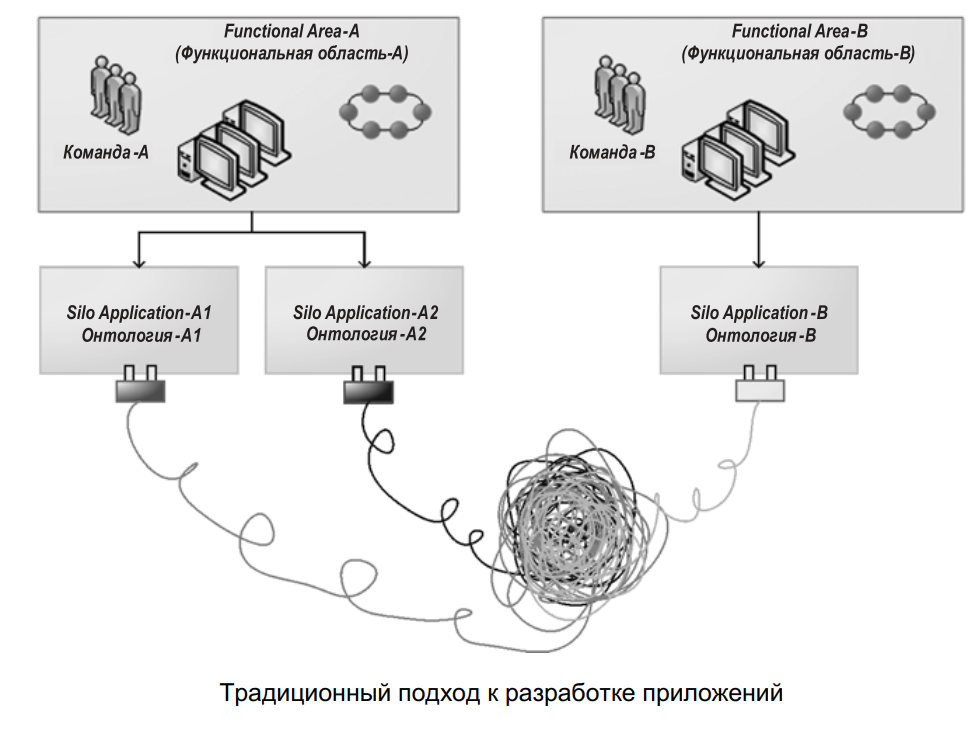
\includegraphics[scale=.5]{./images/problems.png}

\end{frame}

\begin{frame}{OSTIS}
    Использование интеллектуальных технологий - платформа OSTIS является мощным инструментом для создания интеллектуальных информационных систем, способствующих инновационному развитию в различных отраслях, от промышленности до образования и медицины.
\end{frame}
\end{document}
